\chapter{Introdução}
\label{chap:intro}

Nesse estudo foi feita a implementação do algoritmo de planejamento de trajetória Probabilistic Roadmap (PRM) em um robô diferencial não-holonômico chamado Turtlebot3 para permitir a navegação autônoma desse robô. Os testes foram realizados em ambiente de simulação e em um labirinto real construído. 

\begin{figure} [h!]	
  \centering
  \caption{Turtlebot3}
  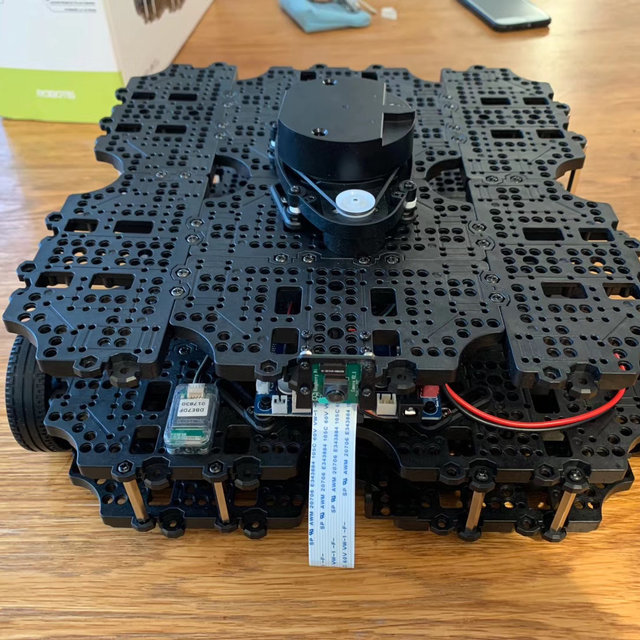
\includegraphics[width=0.6\textwidth,trim={0 1.5cm 0 1.5cm},clip]{Figures/TurtleBot3-Waffle-Pi-robotic-platform_Q640.jpg}
  \caption*{Fonte: Autoria própria.}
  \label{fig:turt1}
\end{figure}

%--------- NEW SECTION ----------------------
\section{Objetivos}
\label{sec:obj}
O objetivo desse estudo foi fazer a implementação do algoritmo de planejamento de trajetória PRM no Turtlebot3 para ser integrada à navegação desse robô como planejador global, a fim de que esse robô pudesse ser capaz de navegar autonomamente em um labirinto, após mapeado, indo de um ponto a outro sem colidir com os obstáculos.
\label{sec:obj}

%--------- NEW SECTION ----------------------
\section{Justificativa}
\label{sec:justi}

Em um trabalho futuro, o algoritmo de planejamento aqui desenvolvido será comparado com outras técnicas de planejamento e trajetória, como A*, D* e Dijkstra, para comparar seus resultados estatisticamente.

%--------- NEW SECTION ----------------------
\section{Organização do documento}
\label{section:organizacao}

Este documento apresenta $5$ capítulos e está estruturado da seguinte forma:

\begin{itemize}

  \item \textbf{Capítulo \ref{chap:intro} - Introdução}: É apresentado o estudo realizado, com a descrição do problema, objetivo e justificativa.;
  \item \textbf{Capítulo \ref{chap:fundteor} - Fundamentação Teórica}: É apresentada a base teórica que sustenta o estudo desenvolvido;
  \item \textbf{Capítulo \ref{chap:metod} - Desenvolvimento do projeto}: Nesse capítulo é apresentado o desenvolvimento realizado para implementar o planejador;
  \item \textbf{Capítulo \ref{chap:result} - Resultados}: Nesse capítulo são apresentados os resultados obtidos;
  \item \textbf{Capítulo \ref{chap:conc} - Conclusão}: Apresenta as conclusões do trabalho e trabalhos futuros.

\end{itemize}
